% theKATRINexperiment.tex
%

    \chapter{KATRIN experiment}
    \label{ch:The KATRIN experiment}
    The KATRIN experiment is on its way to measure the neutrino mass or set new upper limits at precisions never achieved before. It will reach a sensitivity of \SI{200}{\milli\electronvolt}/\SI{}{\square c} at \SI{90}{\percent} C.L. excelling the previously best experiments of Mainz and Troisk by a factor of \SI{10}{}. Major challenges of the project are the requirement of ultra high vacuum, the exact knowledge of all magnetic and electric fields as well as external influences on those, the required high luminosity of the tritium source and the classification and reduction of background sources.
    
      \section{Measurement principle}
      \label{ch:The KATRIN experiment:sec:Measurement Principle}
      A generally easy principle is used to find information on the neutrino mass. The energy of electrons from tritium decay is measured with high precision and compared to the standard model's presumption for a massless neutrino \cite{Otten:2008zz}
      \begin{equation}
      	\ce{^3_1T -> ^3_1H^+ + e^- + \bar{\nu}_e}.
      \end{equation}
      As the decay's energy is distributed between the constant neutrino's rest mass and the neutrino's and the electron's kinetic energies respectively, the decay electrons will show a continuous spectrum. The difference between the electron energy calculated by standard model presumptions and the extrapolated maximum electron energy from the spectrum is extracted. As all three mass eigenstates contribute to the electron neutrino's mass in any scenario (see \ref{ch:Introduction:sec:neutrino Oscillations}, the difference will be a superposition of these. The knees occuring at each single eigenstates mass can not be resolved with the KATRIN spectrometer as the energy resolution is larger than the root of the squared mass differences.
      shown in figure \ref{fig:katrinExperiment:tritiumSpectrum}. As all three flavors contribute to the electron neutrino's mass, what will be measured is the incoherent sum of all three as described in chapter \ref{ch:Introduction:sec:Neutrinos in the standard model}.
      
      \begin{figure}
	\centering
      	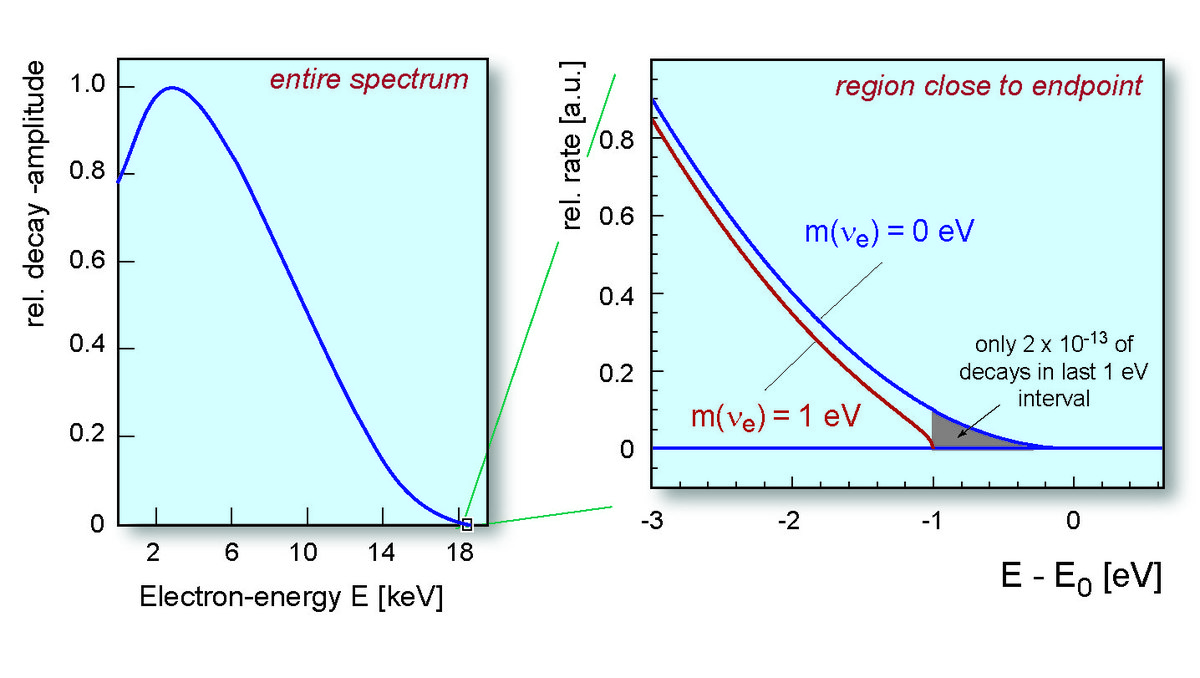
\includegraphics[width = 0.9 \textwidth]{graphics/katrinExperiment/electronSpectrum.jpg}
      	\caption[Schematic tritium energy spectrum]{Schematic energy spectrum for electrons from tritium beta decay. On the left, the entire spectrum with the peak at the energy most emitted - around \SI{5}{\electronvolt} - can be seen. On the right, a zoom-in on the endpoint showing both the calculations for a massless and a \SI{1}{\electronvolt} neutrino. As described in the graph, rates in this region are extremely low and extrapolation through advanced software tools needs to be applied.}
      	\label{fig:katrinExperiment:tritiumSpectrum}
      \end{figure}
      A different light is shed on the simplicity of the task when considering the needed accuracy of $\Delta E < \SI{0.93}{\electronvolt}$ needed for the electrostatic filter to achieve the desired sensitivity \cite{KATRINWolf}. And this is just one in a meshwork of requirements necessary. All components need to work as a whole in the end, not a single one may contribute to the background much more than expected.
       \subsection{MAC-E Filter}
                   \begin{figure}
	\centering
      	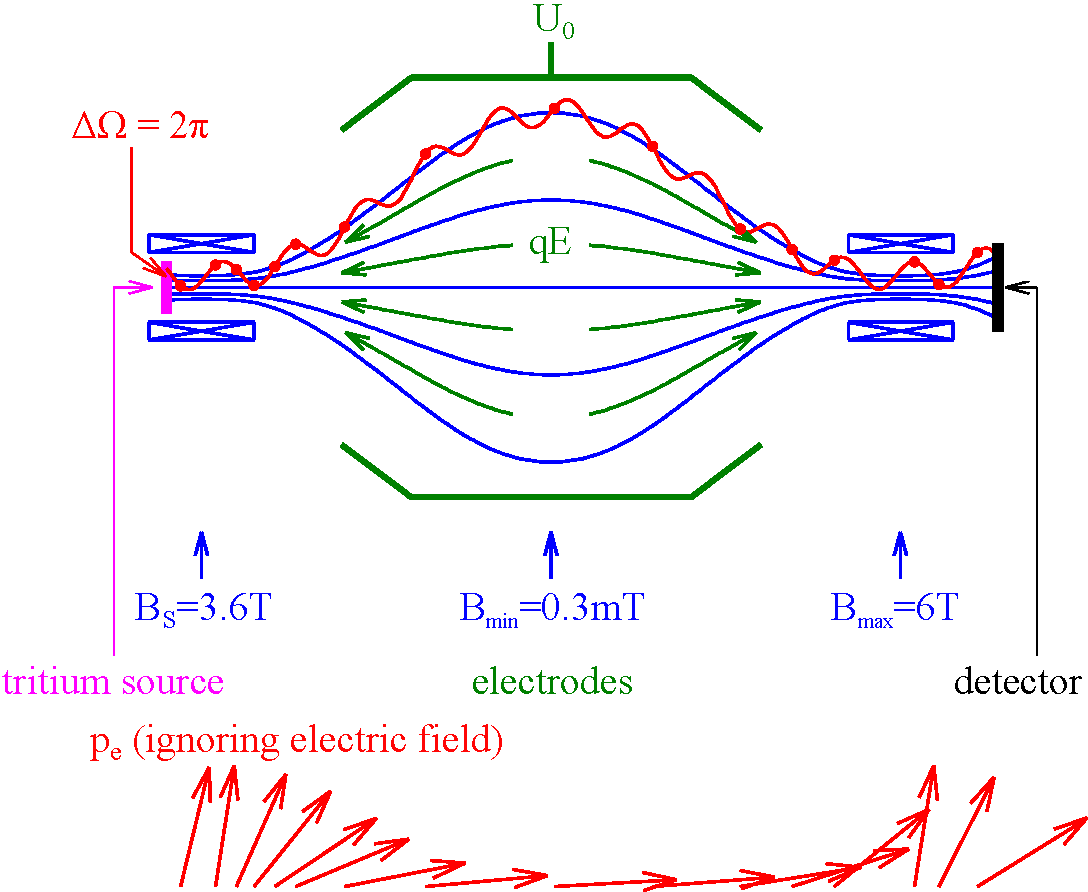
\includegraphics[width = 0.8 \textwidth]{graphics/katrinExperiment/macEFilter.pdf}
      	\caption[MAC E Filter]{Principle of a MAC E filter. In the upper part, magnetic fieldlies are plotted in blue together with fieldstrengths at the source (\SI{3.6}{\tesla}) and inside the pinch solenoid (\SI{6}{\tesla}). The accepted solid angle and a exemplary particle path are shown in red. The analysis plane is defined by the area of minimum magnetic fields $B_{min}$. Below, the momentum of an electron with a large starting angle towards the magnetic field lines is shown. It is tipping over as the field weakens. Meanwhile, the vessel voltage $U_0$ analyses the energy parallel to the electric field passing only electrons with large enough energies on to the detector \cite{macEFilter}.}
      	\label{fig:katrinExperiment:macEFilter}
      \end{figure}
      \label{ch:The KATRIN experiment:sec:MAC-E}
		To measure the energy of electrically charged decay electrons at high precision, an electrostatic filter comes to mind. As the electrons are emitted isotropically, they will have momentum components both parallel and perpendicular to the source-detector axis (defined as the z-axis). To make statements on the overall energy, the momentum direction needs to be well defined. In case of an electrostatic filter, it needs to be parallel to the electric field to be analyzed.
		At the same time, a high luminosity is a major requirement for good statistics for the KATRIN experiment.
		To satisfy all these requirements, several techniques are combined in the MAC-E filter - magnetic adiabatic collimation with electrostatic filter \cite{katrinPrinciple}.\\\\
		{\bf Magnetic} fieldlines connect the source and the detector. Electrons from tritium decays are guided from source side to detector in cyclotron motion around one of these field lines. This strongly raises luminosity as electrons with large angles towards the z axis will not necessarily hit the wall of the source but will be able to reach the detector.\\\\
		{\bf Adiabatic} motion in the magnetic field is defined by the allowance of momentum direction changes at constant momentum value. That is given if the magetic field change is small within each cyclotron orbit. If so, the magnetic momentum $\mu$ correlated to $E_\bot$ (the energy perpendicular to the magnetic field $B$) as follows remains constant
		\begin{equation}
			\mu = \frac{E_{\bot}}{B} = const \propto \frac{p^2_\bot}{B}.
			\label{eq:magMomentum}
		\end{equation}
		{\bf Collimation} in a MAC-E filter is based on the above adiabacity. Magnetic field strengths drop over several orders of magnitude from $B_{max}$ at the solenoid magnets to $B_{min}$ in the analysis plane (see figure \ref{fig:katrinExperiment:macEFilter}). Considering equation \ref{eq:magMomentum}, this means that the energy perpendicular to the magnetic field must drop over the same order of magnitude for $\mu$ to remain constant. This leads to a parallelization of momentum vector and B-field direction. \\\\
		{\bf Electrostatic filtering} occurs exactly at that point of minimal energies $E_\bot$ in the analysis plane. Here, the momentum vector is mostly defined by its component parallel to the magnetic field $E_{||}$. Setting the electrostatic filter to a fixed voltage $U$ now reflects electrons with $E_{||} < U\cdot e$.\\
		Most electrons are emitted at the source are non-parallel to the magnetic field lines and thus an energy $E_\bot \neq 0$. That means that it is very likely that electrons in the analysis plane have remaining energy $E_\bot$. This limits the filter resolution, with 
		\begin{equation}
			\mu_{low} = \frac{E_{\bot_{min}}}{B_{min}} = \frac{E_{\bot_{max}}}{B_{max}} = \mu_{high} = \mu
		\end{equation}

		the relative sharpness is given by the maximum transversal energy $E_{\bot_max}$ that is still accepted in the filter. As for a 
		\begin{equation}
		\Delta E = E_{\bot_{max}} = E_{0}\frac{B_{min}}{B_{max}}
% 			\frac{\Delta E}{E} = \frac{B_{min}}{B_{max}}.
		\end{equation}
		
		Only in the edge case of $B\rightarrow 0$ in the analysing plane, the momentum would need to be exactly parallel to the field and the resolution would not be limited.
		After passing the analysing plane, the electrons are reaccelerated by the electric field and guided and focused onto a detector.
		To additionally dismiss electrons with large starting angles towards the magnetic field, the source field strengthsare chosen to be smaller than the maximum field strength inside the solenoid. This ensures that electrons with long paths that are more likely to scatter will not be analyzed through the effect of magnetic mirroring \cite{magneticMirror}.
		With the chosen settings, this results in an angular acceptance of \SI{50.77}{\degree}. The main spectrometer reaches a resolution of \SI{0.93}{\electronvolt} (see section \ref{ch:The KATRIN experiment:sec:Experimental setup:subsec:MainSpec} for more details).
% 		\begin{equation}
% 			\mu_{\mathrm{0}} = \mu_{\mathrm{low}} ~ \longrightarrow ~ \frac{E_{\bot_0}}{B_0} = \frac{E_{\bot_{low}}}{B_{low}} 
% 		\end{equation}
%       To further filter out electrons with high starting angle, the source is set to lower fields than the maximum $B_{max}$.
%       As with larger angles come longer paths, this reduces the probability of electrons taking part in scattering processes inside the source section being detected.
%       \begin{equation}
%       	\theta_{s~max}= \arcsin{\sqrt{\frac{B_s}{B_{max}}}}
%       \end{equation}
%       

      

      \section{Experimental Setup}
      \label{ch:The KATRIN experiment:sec:Experimental setup}
      The KATRIN experiment is made up of different sections all fulfilling their own important purpose in the whole setup. All begins at the windowless gaseous tritium source ``WGTS''. Here, tritium decays isotropically emitting electrons. These are guided magnetically through the differential and cryogenic pumping sections ``DPS'' and ``CPS'' removing hydrogen ions and other residual gases in the process. At the same time, looking at the WGTS from the other direction, the rear section scans the activity of the source. For the electrons on their way to the detector, the path continues through the two spectrometers posing as a energetic high pass filter to the focal plane detector ``FPD'' registering them.\\
      During the whole procedure, the electrons from the decay may not undergo energy changes as the knowledge of their kinetic energy after decaying is essential to the experiment. That is why the guiding needs to be adiabatic. This is guaranteed by spatially slowly changing and timewise very constant magnetic fields.\\
      See figure \ref{fig:beamLine} for a schematic overview of the whole experimantal setup. It follows a more detailed description of the individual components.
      
      \begin{figure}
			
      		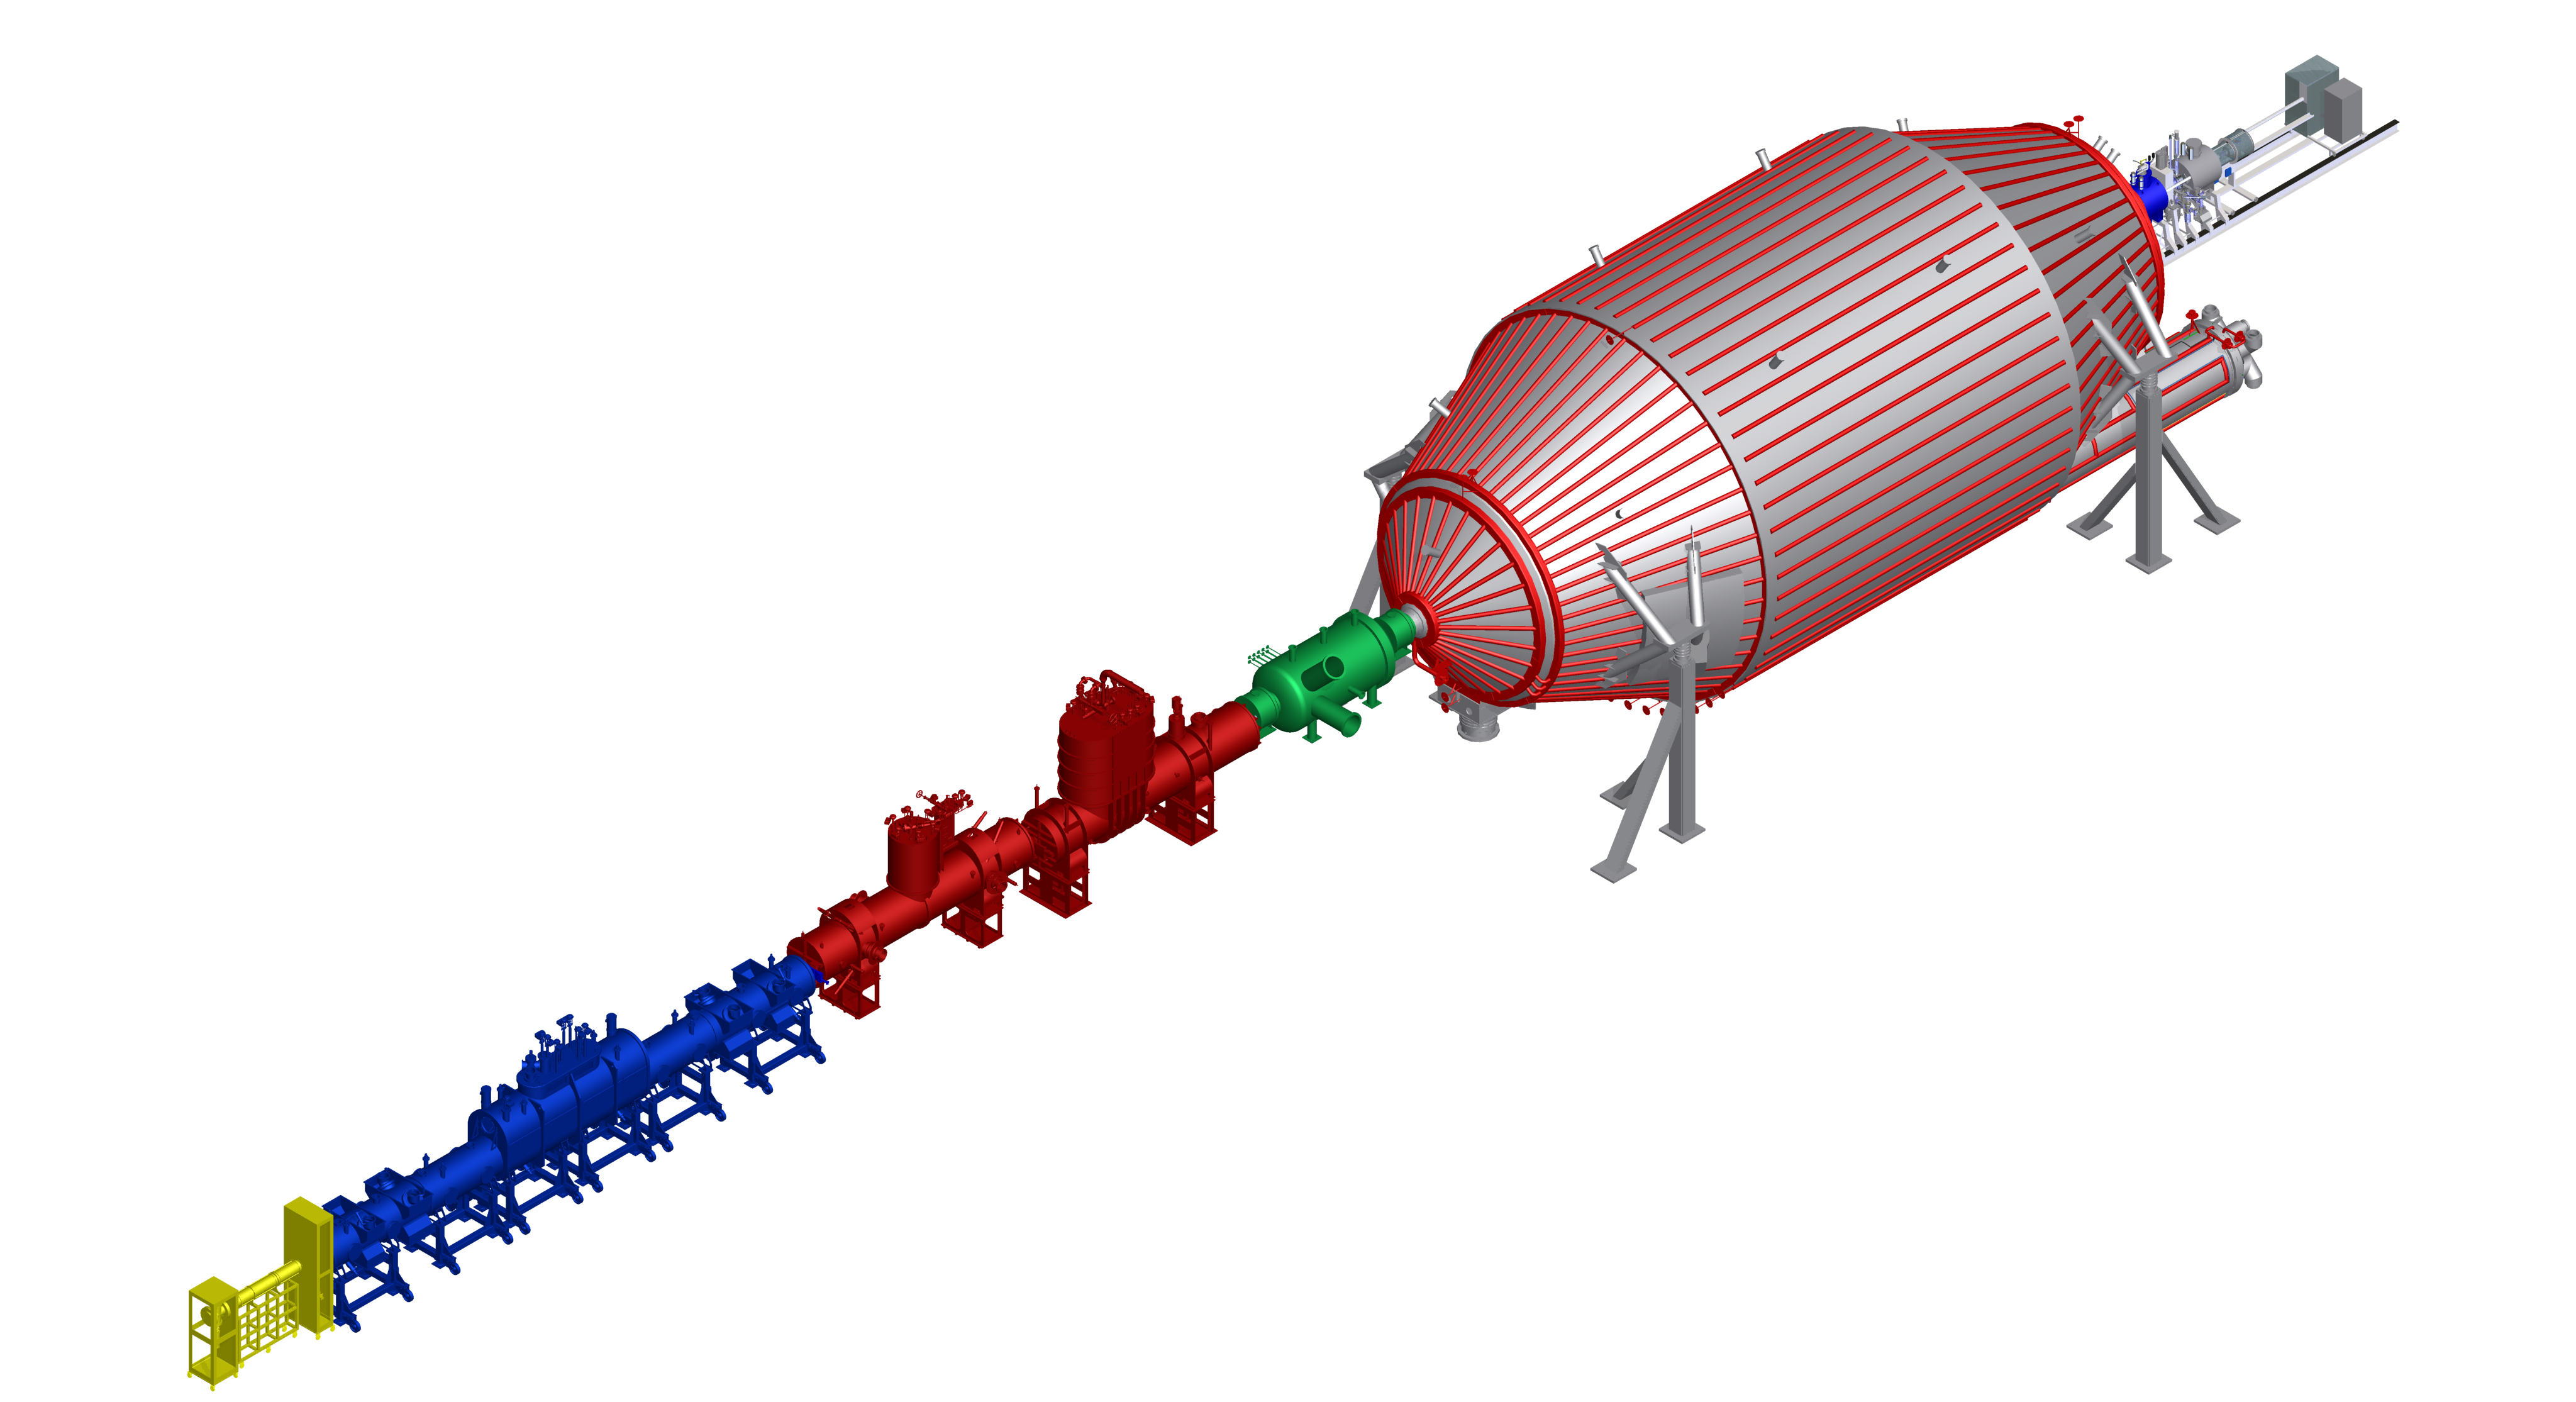
\includegraphics[width = \textwidth]{graphics/katrinExperiment/beamLineHD.jpg}

      	\caption[KATRIN beam line]{The beam line of the KATRIN experiment with the different stages: Rear section (yellow) and WGTS (blue) on the very left, followed by the transport section (red) consisting of DPS and CPS. Energy analysis in pre- (green) and main spectrometer (grey-red) of the spectrometer section and electron detection at the detector section (grey-blue).}
      	\label{fig:beamLine}
      \end{figure}

      
      \subsection{WGTS and Rear Section}
      \label{ch:The KATRIN experiment:sec:Experimental setup:subsec:sourceSide}
      To generate tritium decay electrons, a gaseous tritium source is utilized (see figure \ref{fig:sourceSide}). Advantages of the principle are the absence of solid state effects and a high luminosity \cite{letterOfIntent}. In a solid, like tritium films, most electrons from decays inside the structure would interact with the solid itself. That could lead to energy shifts threatening the energy resolution. Another advantage of using a gaseous source is that not only the surface facing the detector emits electrons at the required spectrum, but the electrons from the whole volume covered by the magnetic flux tube hitting the detector can be analyzed. Furthermore, the emission of this kind of source is very homogeneous. Of course, new challenges arise from the decision to use gas instead of solids.
      \begin{itemize}
		\item The source's temperature needs to be very robust (max. \SI{\pm0.03}{\kelvin} at \SI{30}{\kelvin}) to guarantee a rate stability of \SI{\pm0.1}{\percent} for the decay electrons \cite{temperatureWGTS}.
      	\item The spectrometers further downstream require for ultra high vacuum, for the main spectrometer in the order of \SI{e-11}{\milli\bar}. With the tritium pressure is in the order of \SI{10e-3}{\milli\bar} and the source's need to be windowless - no electron transparent window is known to stand such pressure differences - the pressure must be reduced to desired values without any physical barrier.
      	\item The tritium isotope contributions of the gas need to be known precisely, for that purpose a laser-raman-system has been developed \cite{calibrationRaman}.
      	\item All devices used in contact with tritium have to undergo excessive testing in tritium environment to fault failure safety under the harsh conditions.
      \end{itemize}
      
     \begin{figure}
     \centering
		\begin{minipage}{0.6\textwidth}
				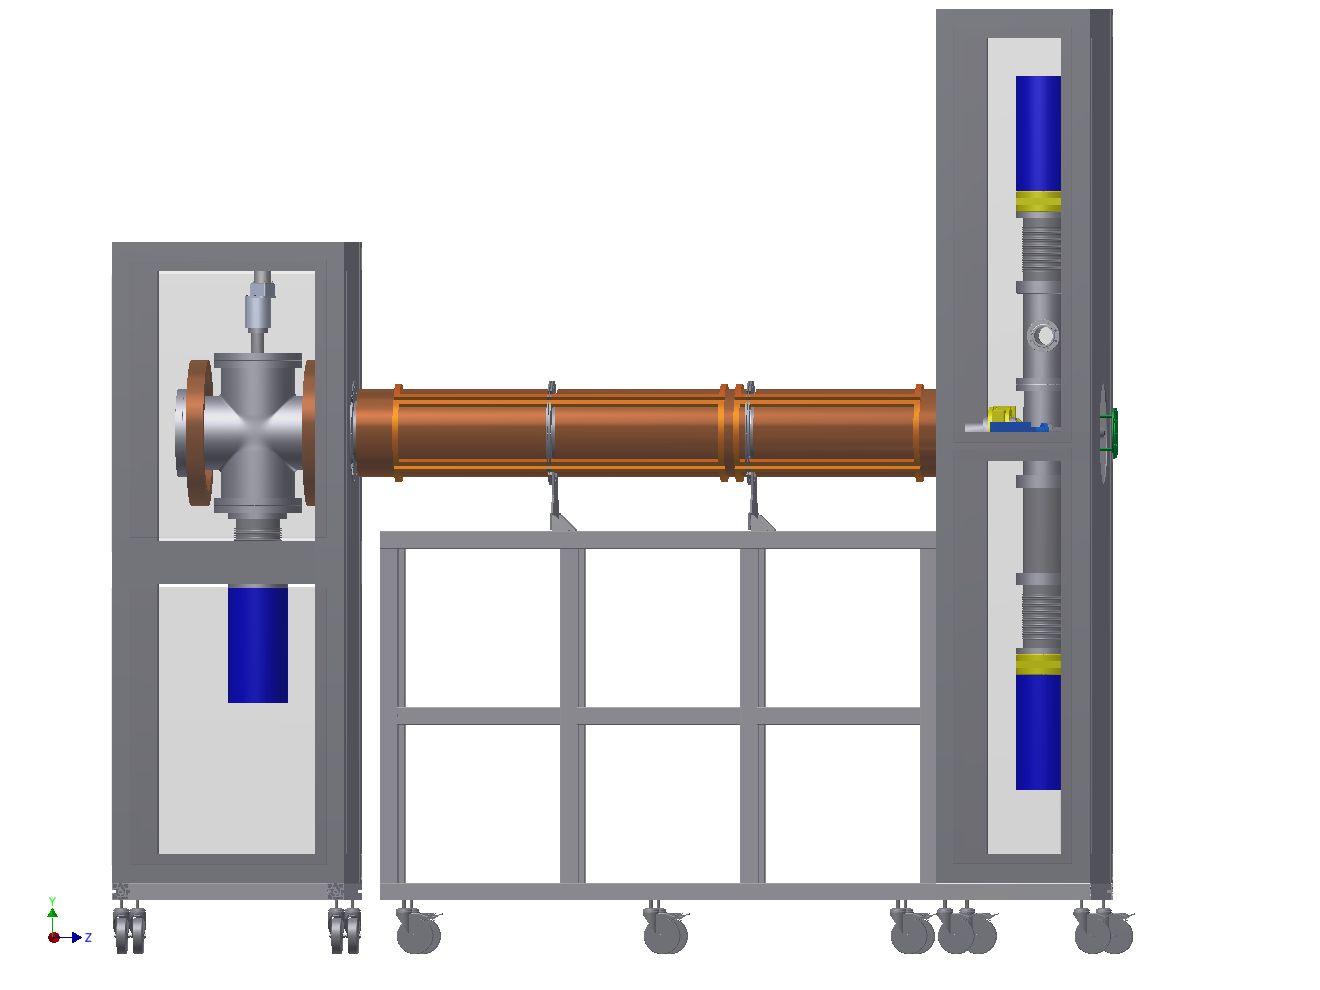
\includegraphics[width = 1.0\textwidth]{graphics/katrinExperiment/rearSectionFull1.png}
		\end{minipage}
		\begin{minipage}{\textwidth}
			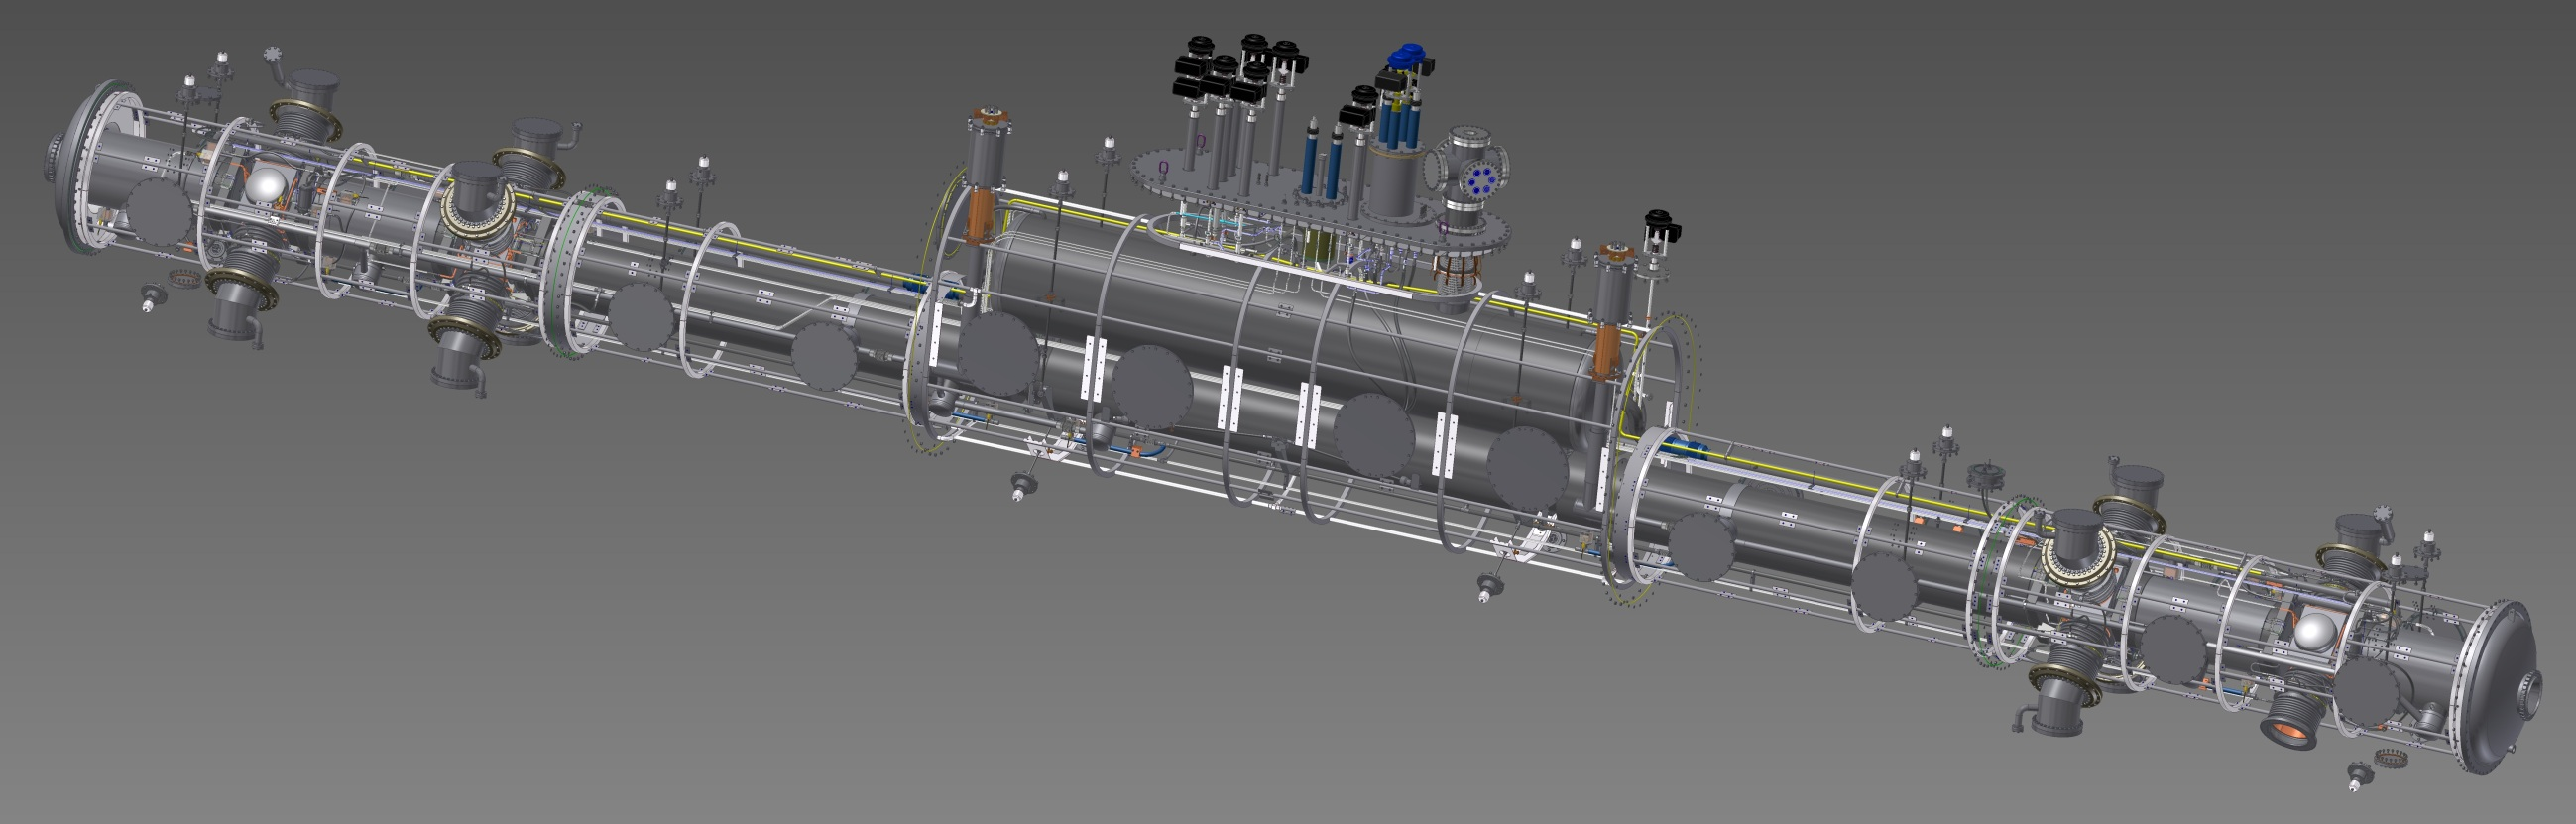
\includegraphics[width = 1.0\textwidth]{graphics/katrinExperiment/WGTS.jpg}
		\end{minipage}
		\caption[Rear section and WGTS]{On top, the rear section. In the model, there are two large attachments visible perpendicular to beam direction. The right one is the e-gun for calibration purposes. LEFT ONE!!!!. Also visible are the gray second containment boxes making for redundancy in radiation security. Below a model of the WGTS. The many pumping ports are clearly visible on the left and the right end, in the wider, middle section tritium is injected. Images from \cite{rearSection} and \cite{WGTSDrexlin}}.
		\label{fig:sourceSide}
      \end{figure}
      
      
      \subsection{Transport and Pumping Section}
      
      In the DPS, pressure is actively reduced by seven orders of magnitude with the use of turbo molecular pumps. These as well need to be tested thoroughly to withstand the constant radiation by tritium decays \cite{tritiumTests}. The tritium gas is then processed to be reused in the tritium cycle. Further downstream, the CPS uses strongly cooled walls to freeze residual gas, always keeping the information carrying electrons away from those by magnetic guidance. 
      \begin{figure}
		\begin{minipage}{0.49\textwidth}
				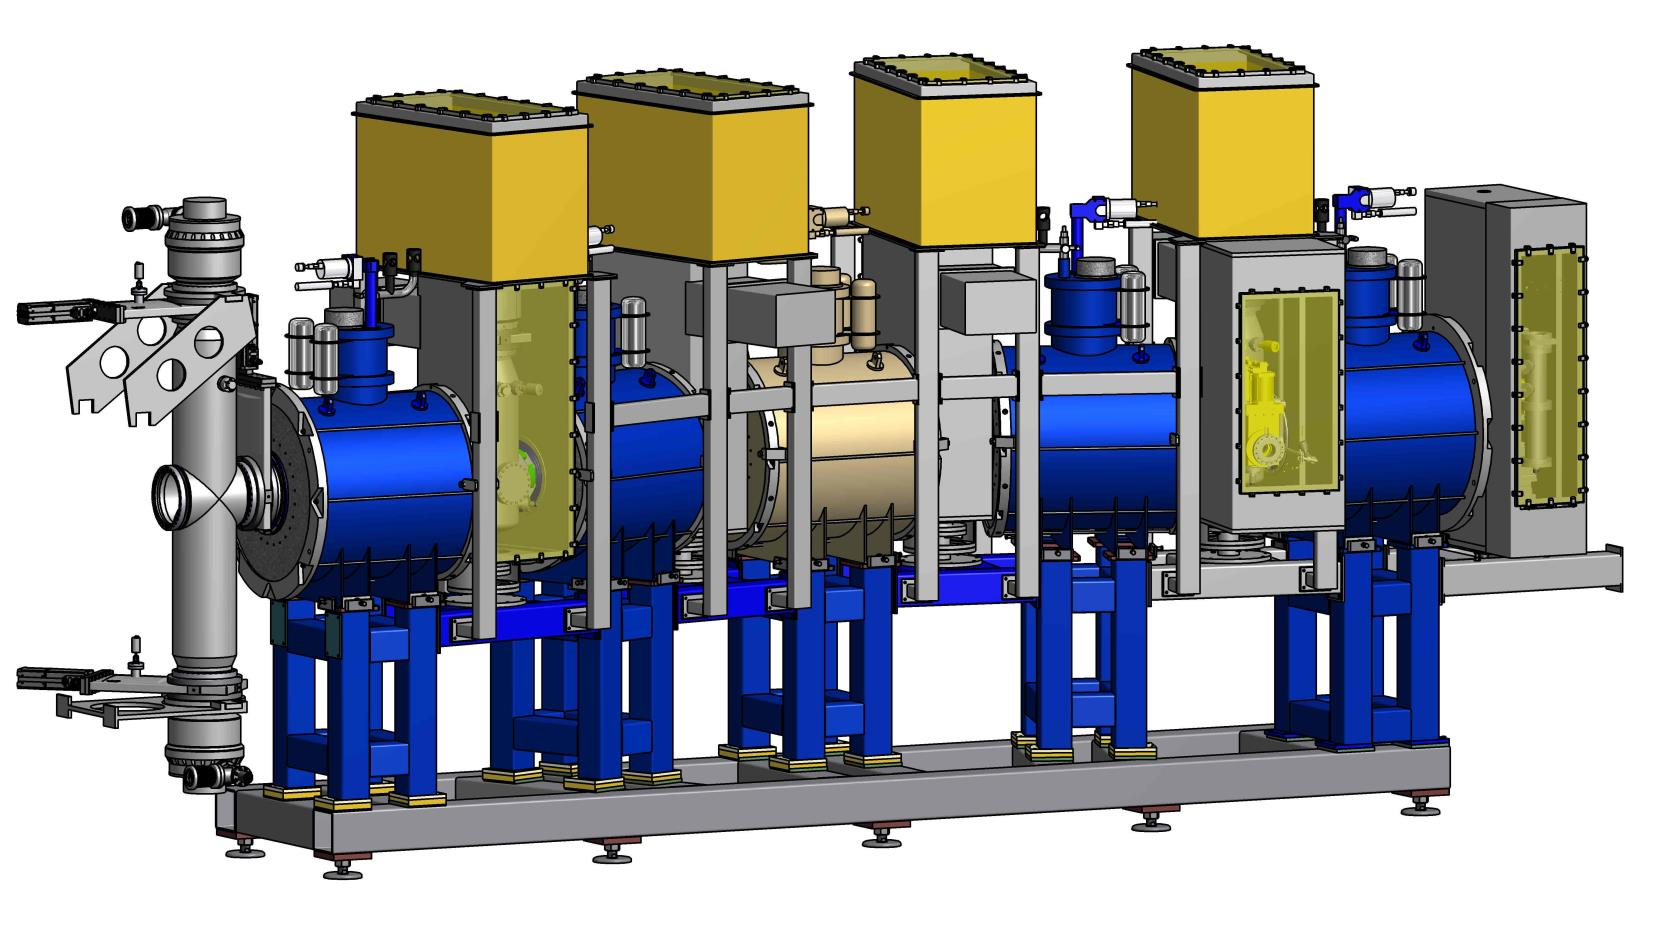
\includegraphics[width = 1.0\textwidth]{graphics/katrinExperiment/DPS.jpg}
		\end{minipage}
		\begin{minipage}{0.49\textwidth}
			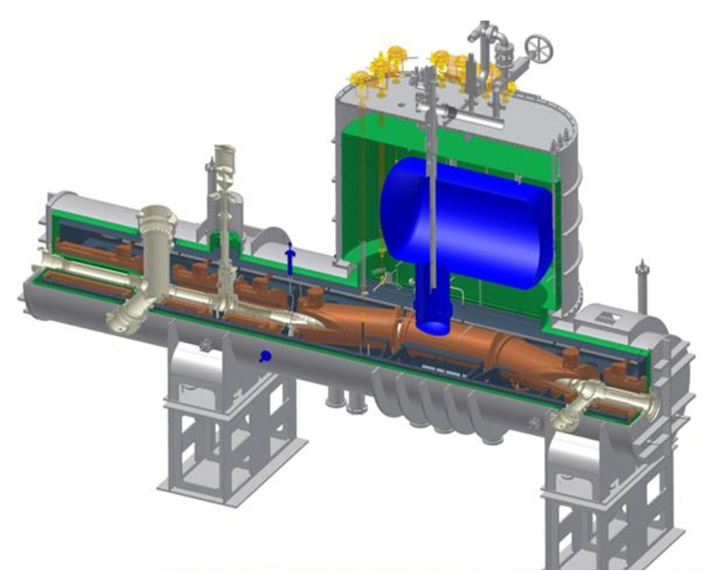
\includegraphics[width = 1.0\textwidth]{graphics/katrinExperiment/CPS.jpg}
		\end{minipage}
		\caption[DPS and CPS]{Differential and cryogenic pumping sections, left the DPS with pumping ports all over the structure. All of the ports are isolated against the surroundings (yellow boxes) to protect against potential radiation leaks. On the right the CPS with its coolable wall structure to capture free particle as well as standard pumping ports \cite{DPS, CPS}.}
      \end{figure}
      
      \subsection{Pre-Spectrometer}
      \label{ch:The KATRIN experiment:sec:Experimental setup:subsec:PreSpectrometer}
      The pre-spectrometer was built to reduce the flux to the main spectrometer by ~7 orders of magnitude \cite{statusPSWolf}. It works on the MAC-E filter principle from chapter \ref{ch:The KATRIN experiment:sec:MAC-E}. Being a lot smaller, its energy resolution can of course not compete with the main spectrometer one. Its purpose is to cut off the spectum below energies of \SI{18.4}{\kilo\electronvolt}, the electrons above that limit will pass and be further analyzed in the main spectrometer. Here, it is important that the momentum is restored after analysis which requires for a symmetric setup. To shield against externally induced electrons, the pre-spectrometer has a single layer of wires as a inner electrode. It can be set to negative voltages in comparison to the pre-spectrometer hull which then reflects electrons with energies up to $Ue$.
      
      \subsection{Main Spectrometer}
      \label{ch:The KATRIN experiment:sec:Experimental setup:subsec:MainSpec}
      The largest component of all is the main spectrometer. With a diameter of \SI{10}{\meter} and a length of over \SI{23}{\meter}, it incorporates around \SI{1400}{\cubic\meter} that need to be evacuated to extremely high vacuum of < \SI{e-11}{\milli\bar}. The main spectrometer, as the pre spectrometer, makes use of MAC-E filtering technique from \ref{ch:The KATRIN experiment:sec:MAC-E}. To do so, it features a uniquely designed electrode and a high voltage system \cite{mainSpecElectrodeDesign}. A precision voltage divider was constructed to read out the high voltage applied to the vessel with the highest precision voltmeters, which operate in the order of \SI{10}{\volt} \cite{highVoltageDivider}. Additionally, the voltage is fed to the monitor spectrometer from section \ref{ch:TheKATRINexperiment:sec:experimentalSetup:subsec:monSpec} to ensure its long term stability.
      
      The vessel is equipped with two layers of electrodes on a comb-like structure. This setup reduces the number of secondary electrons from the spectrometer walls entering the flux tube's volume. Keeping that count low, the rate of those electrons not reflected magnetically due to imperfect symmetries is reduced to the sub-\SI{}{\electronvolt} level \cite{wireElectrodeSystem}. The layer made from thinner wires further to the inside shields the spectrometer volume from the one further towards the wall as cosmic rays may unleash electrons there as well.
      The main spectrometer as a whole is set to high voltage varied in the region below the endpoint of ~\SI{18.6}{\kilo\volt}. It constitutes the MAC-E filter from \ref{ch:The KATRIN experiment:sec:MAC-E}. The wire electrodes float on that voltage with a added more negative value to shield against electron background.
      \begin{figure}
      
      	\begin{minipage}{0.67\textwidth}
      		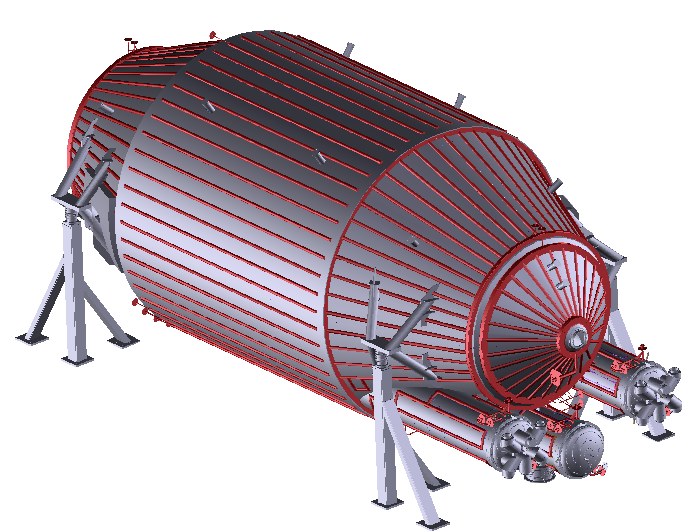
\includegraphics[width = \textwidth]{graphics/katrinExperiment/mainSpectrometer.jpg}
      	\end{minipage}
      	\begin{minipage}{0.29\textwidth}
      		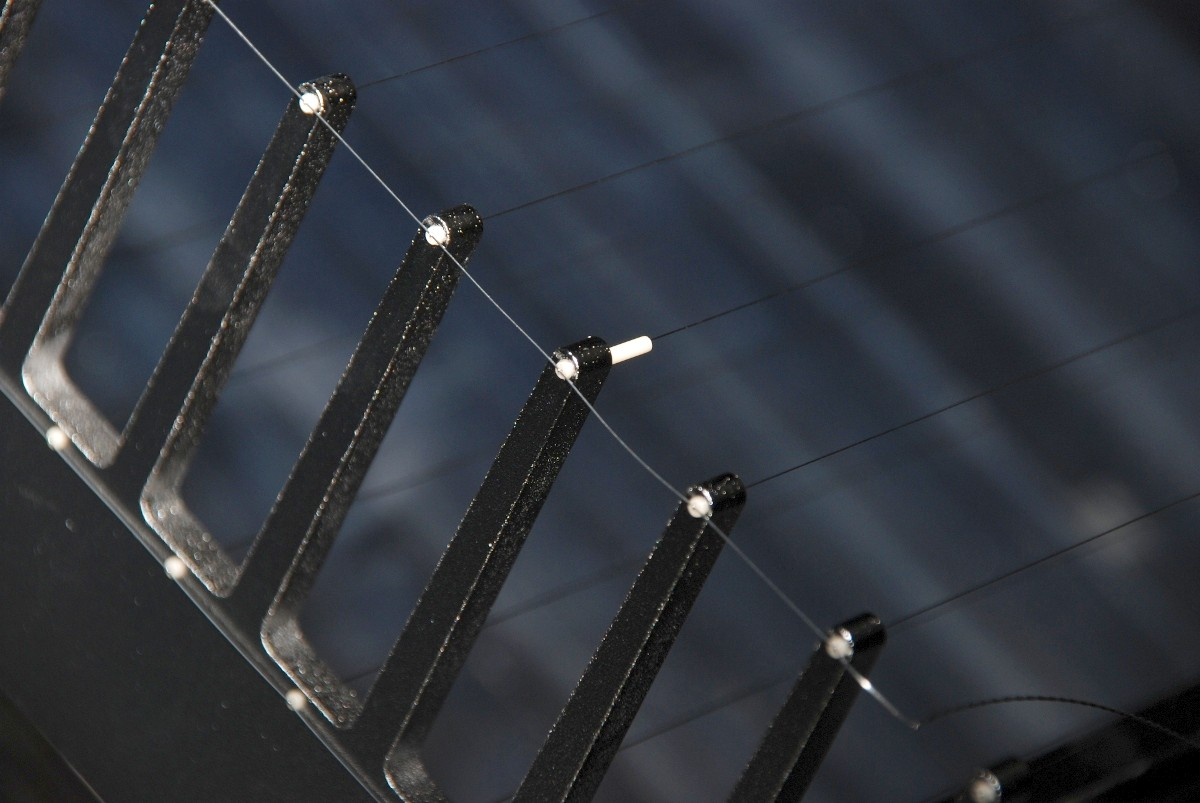
\includegraphics[angle = 90, width = \textwidth]{graphics/katrinExperiment/wireElectrodes.png}
      	\end{minipage}
      	\caption[Main spectrometer and wire electrodes]{On the left, the main spectrometer of the KATRIN experiment \cite{mainSpecStatus}. It is divided into a central, cylindric shape to which two flat cones, disemboguing in the steep cones, are attached. Also visible in this image are the 3 large pump ports on the lower right and the three-legged holding structures. On the right a image of the comb structure of the inner electrodes with both layers of wires visible. The white structures on both top and bottom of the combs are the insulation of the wires \cite{collabWireElectrodes}.}
      	\label{fig:mainSpec}
      \end{figure}
		
      \subsection{Monitor spectrometer}
      \label{ch:TheKATRINexperiment:sec:experimentalSetup:subsec:monSpec}
      
      The third MAC-E filter at KATRIN is the slightly modified Mainz spectrometer. It has been transported to Karlsruhe to work as a high voltage monitoring device. Here, electrons from $^{83m}$ Kr decays are detected and analyzed. The fact that the energy from these decays does not change over time (neglecting changes in the source material) can be used to detect shifts in the voltage of the MAC-E filter. For that purpose, the monitor spectrometer constantly measures transmission functions of 
      The monitor spectrometer features two scintillation modules for muon detection that were used for a first inspection of muon induced background.

     
      \subsection{Focal Plane Detector System}
      \label{ch:The KATRIN experiment:sec:Experimental setup:subsec:FPD system}
      The detector is located at the very north of the experiment. It is made up of a silicon wafer whose back-side is divided into 148 pixels attached to the readout electronics by pin connectors. The pattern is dartboard-like, multiple pixels with the same distance to the center form rings. Every pixel has the same surface area, making rates more easily comparable - that is for a magnetic flux through the wafer as homogeneous as in this experiment.
      The detector system is roughly divided into two chambers: one connected to the ultra high vacuum of the main spectrometer and one with a lower grade vacuum on the detectors readout side.
      
      
      \begin{figure}
      \centering
	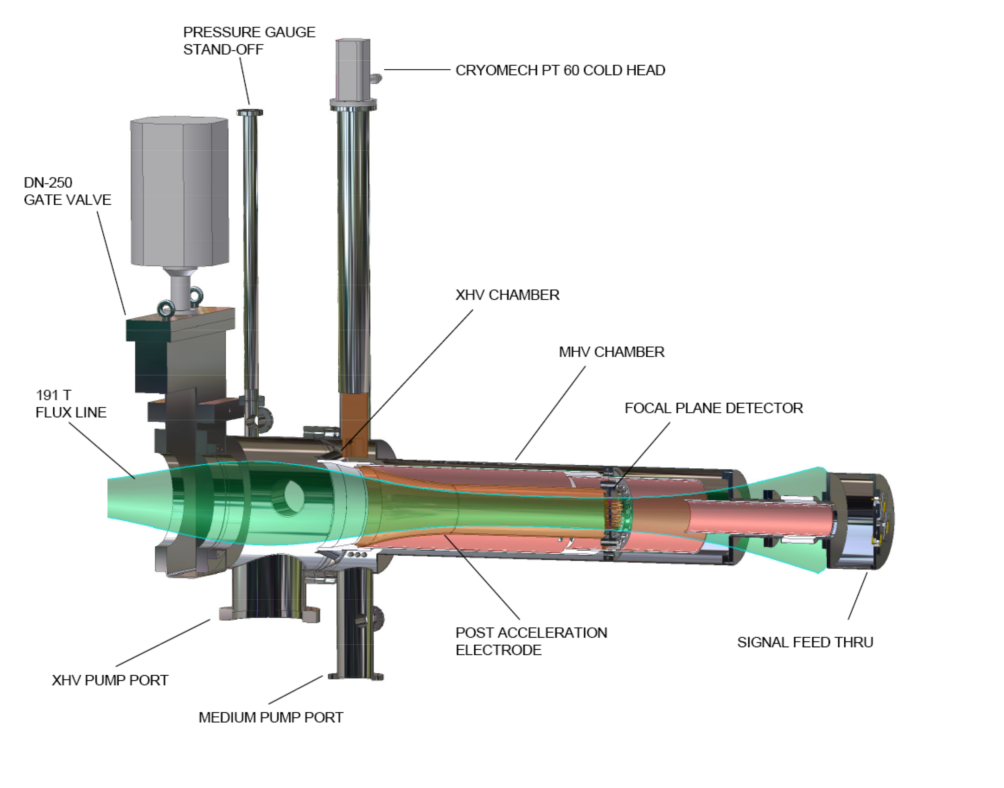
\includegraphics[width = 0.8 \textwidth]{graphics/katrinExperiment/detectorHousing.pdf}
	\caption[Focal plane detector system]{The focal plane detector system including a flux tube (green). One can make out the different grade vacuum sections: extremely high vacuum (XHV) and medium high vacuum (MHV). The post acceleration electrode is visible left of the bronze colored actual detector and its signal feed trough on the very right. Multiple flanges and connectors are shown, not included in this picture are the calibration source holders \cite{FPD}.}
	\label{fig:katrinExperiment:detectorHousing}
      \end{figure}
      
      \begin{figure}
      \centering
      	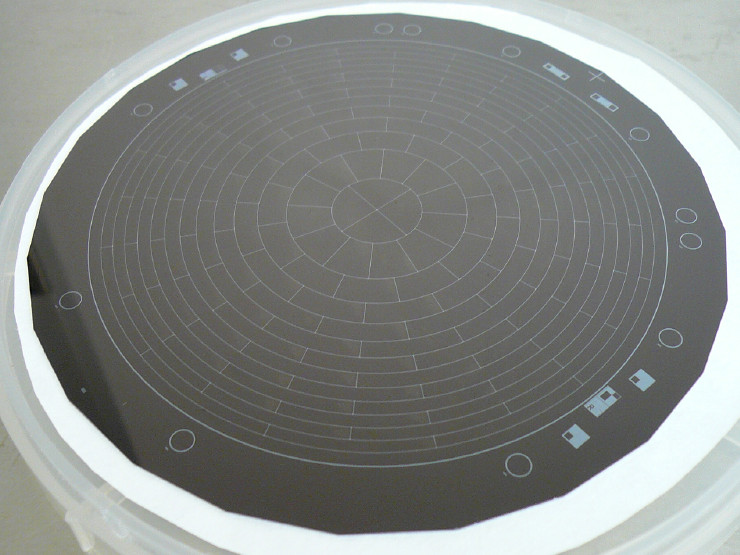
\includegraphics[width = 0.7 \textwidth]{graphics/katrinExperiment/detectorWafer.jpg}
	  \caption[Detector wafer]{The detector wafer as installed in the FPD system. Note the ``dartboard pattern'' with the four pixel bullseye in the center. This is the detectors back side to which the electronics are attached, the front is plaid making for high detection efficiencies.}
	  \label{fig:katrinExperiment:detectorWafer}
      \end{figure}
      
      
      For background reduction, the detector system features both a passive shielding and an active veto system read out by the same data crate as the detector itself. It allows to discriminate against externally induced detector events. Due to the high magnetic fields from detector and pinch magnet, semiconductor readout electronics had to be used instead of conventional photomultiplier tubes.
      As it may be necessary to investigate electrons with energies below the detector threshold, especially for background investigations, a post acceleration electrode has been installed - also visible in \ref{fig:katrinExperiment:detectorHousing} that can add to the electrons' energies through an electric field of known strength.
      
      \subsection{Solenoids, LFCS and EMCS system}
      \label{ch:The KATRIN experiment:sec:Experimental setup:subsec:Solenoids, LFCS and EMCS system}
      
      To achieve magnetic guidance as explained in chapter \ref{ch:The KATRIN experiment:sec:Experimental setup:subsec:Solenoids, LFCS and EMCS system}, a sophisticated system of superconducting solenoids, the low field correction system LFCS and the earth magnetic field compensation system EMCS have been installed \cite{airCoilSystem}. These make sure that the path of flight is kept away from the wall and can be considered adiabatic, that penning traps are avoided as far as possible, that the earth magnetic field is compensated for and, most importantly, that the field drop to the analysis plane is of the order of \todo{order?} so the spectrometers resolution will achieve desired values.
      

      \subsection{Background sources}
      \label{ch:The KATRIN experiment:sec:Experimental setup:subsec:BackgroundSources}
      Different sources contribute to the background of electrons arriving at the detector. Background due to stored electrons is probably the largest source of detector background \cite{storedElectrons}. Penning traps cause electrons with energies in a certain range to be caught in a potential cup. Discharges of those traps due to scattering processes with either residual gas or due to excessive filling of the trap can cause high-rate events at the detector. This can be both dangerous for the detector itself as it is may inhibit data taking. Stored electrons can be both from external sources as from within the spectrometer. Decays of residual gas or wall absorbed molecules can contribute to the background. One large background source is radon, a neutral particle enabling it to move freely inside the vessel. Radon alpha decays, but shakeoff-, conversion- and auger electrons can be guided to the detector from inside the flux tube \cite{radonGoerhard, radonWandkowsky}.
      Another large background source are cosmic rays interacting with the vessel hull and producing electrons like that. This background is reduced mainly by two factors, the symmetry of the magnetic field and the wire electrodes shielding the flux tube up to a certain threshold energy.
      To if the fields, both electric and magnetic, were perfectly symmetrical and parallel, only particles generated within the flux tube would be guided towards the detector. But through inhomogeneities and alignment errors, electrons may enter the flux tube even if generated externally, e.g at the spectrometer wall through $E\times B$ drifts. To keep this from happening, the wire electrodes, were installed. They shield the flux tube against electrons with energies up to $E_e = eU_{wire}$ depending on the wire electrodes voltage $U_{wire}$. 
      \begin{figure}
		\centering
		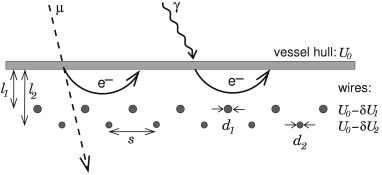
\includegraphics[width = 0.6\textwidth]{graphics/katrinExperiment/wireElectrodes.jpg}
		\caption[Wire electrodes]{A graph of the wire electrodes installed inside the main spectrometer. Both layers of electrodes with different distances to the spectrometer wall are visible, the inner being smaller in diameter than the outer one.}
	  \end{figure}